\thispagestyle{fancy}
% Leave Left and Right Header empty.
\lhead{}
\rhead{}
\renewcommand{\headrulewidth}{1pt}
\renewcommand{\footrulewidth}{0pt}
\newcommand{\packageName}{\textit{SNTD}}

\fancyfoot[C]{}

\pagestyle{fancy}
\lhead{\bf SC NASA EPSCoR GRA    \  $\|$}
\rhead{\bf Justin D. Roberts-Pierel, University of South Carolina}

Observing and understanding gravitationally lensed objects is a new and exciting field of study. The first example of a strongly lensed supernova (SN) resolved into multiple images was SN ``Refsdal'' in 2014 (Kelly et al. 2015). Subsequent work was done to classify Refsdal, as well as to measure time delays and magnification ratios (Rodney et al. 2016). To date, there is no optimally designed software package to analyze correlated data sets from multiply imaged lensed SNe and simultaneously determine SN class, time delays, and magnification ratios. The lack of a standard resource leaves researchers to write and implement their own ad hoc programs, which increases uncertainty and decreases efficiency. In September 2016, the Palomar Transient Factory (PTF) collaboration reported the detection of the first strongly lensed type Ia SN (Goobar et al. 2016), which is an extremely valuable resource to research ranging from lens modeling to constraining cosmic expansion. As these objects will be found with increasing frequency in the future, having a standard software package with the ability to quickly and effectively analyze light curve data for time delay and magnification ratio measurements will be essential (Mesinger and Johnson 2016). In addition, the James Webb Space Telescope (JWST) and Wide Field InfraRed Survey Telescope (WFIRST) era of observations will create still other uses for such a software package, namely applying it to population III (POP III) SN detections. Recent work suggests low-mass POP III and pair instability (PI) SNe will be detectible by JWST and WFIRST, with progenitor masses inferable from light curves (Magg et al. 2016). It's clear that an optimized software package with the ability to analyze a light curve for redshift, SN classification, and other parameters would be extremely valuable to a wide range of research using current and next generation telescopes. 
\begin{figure*}[h]
\centering
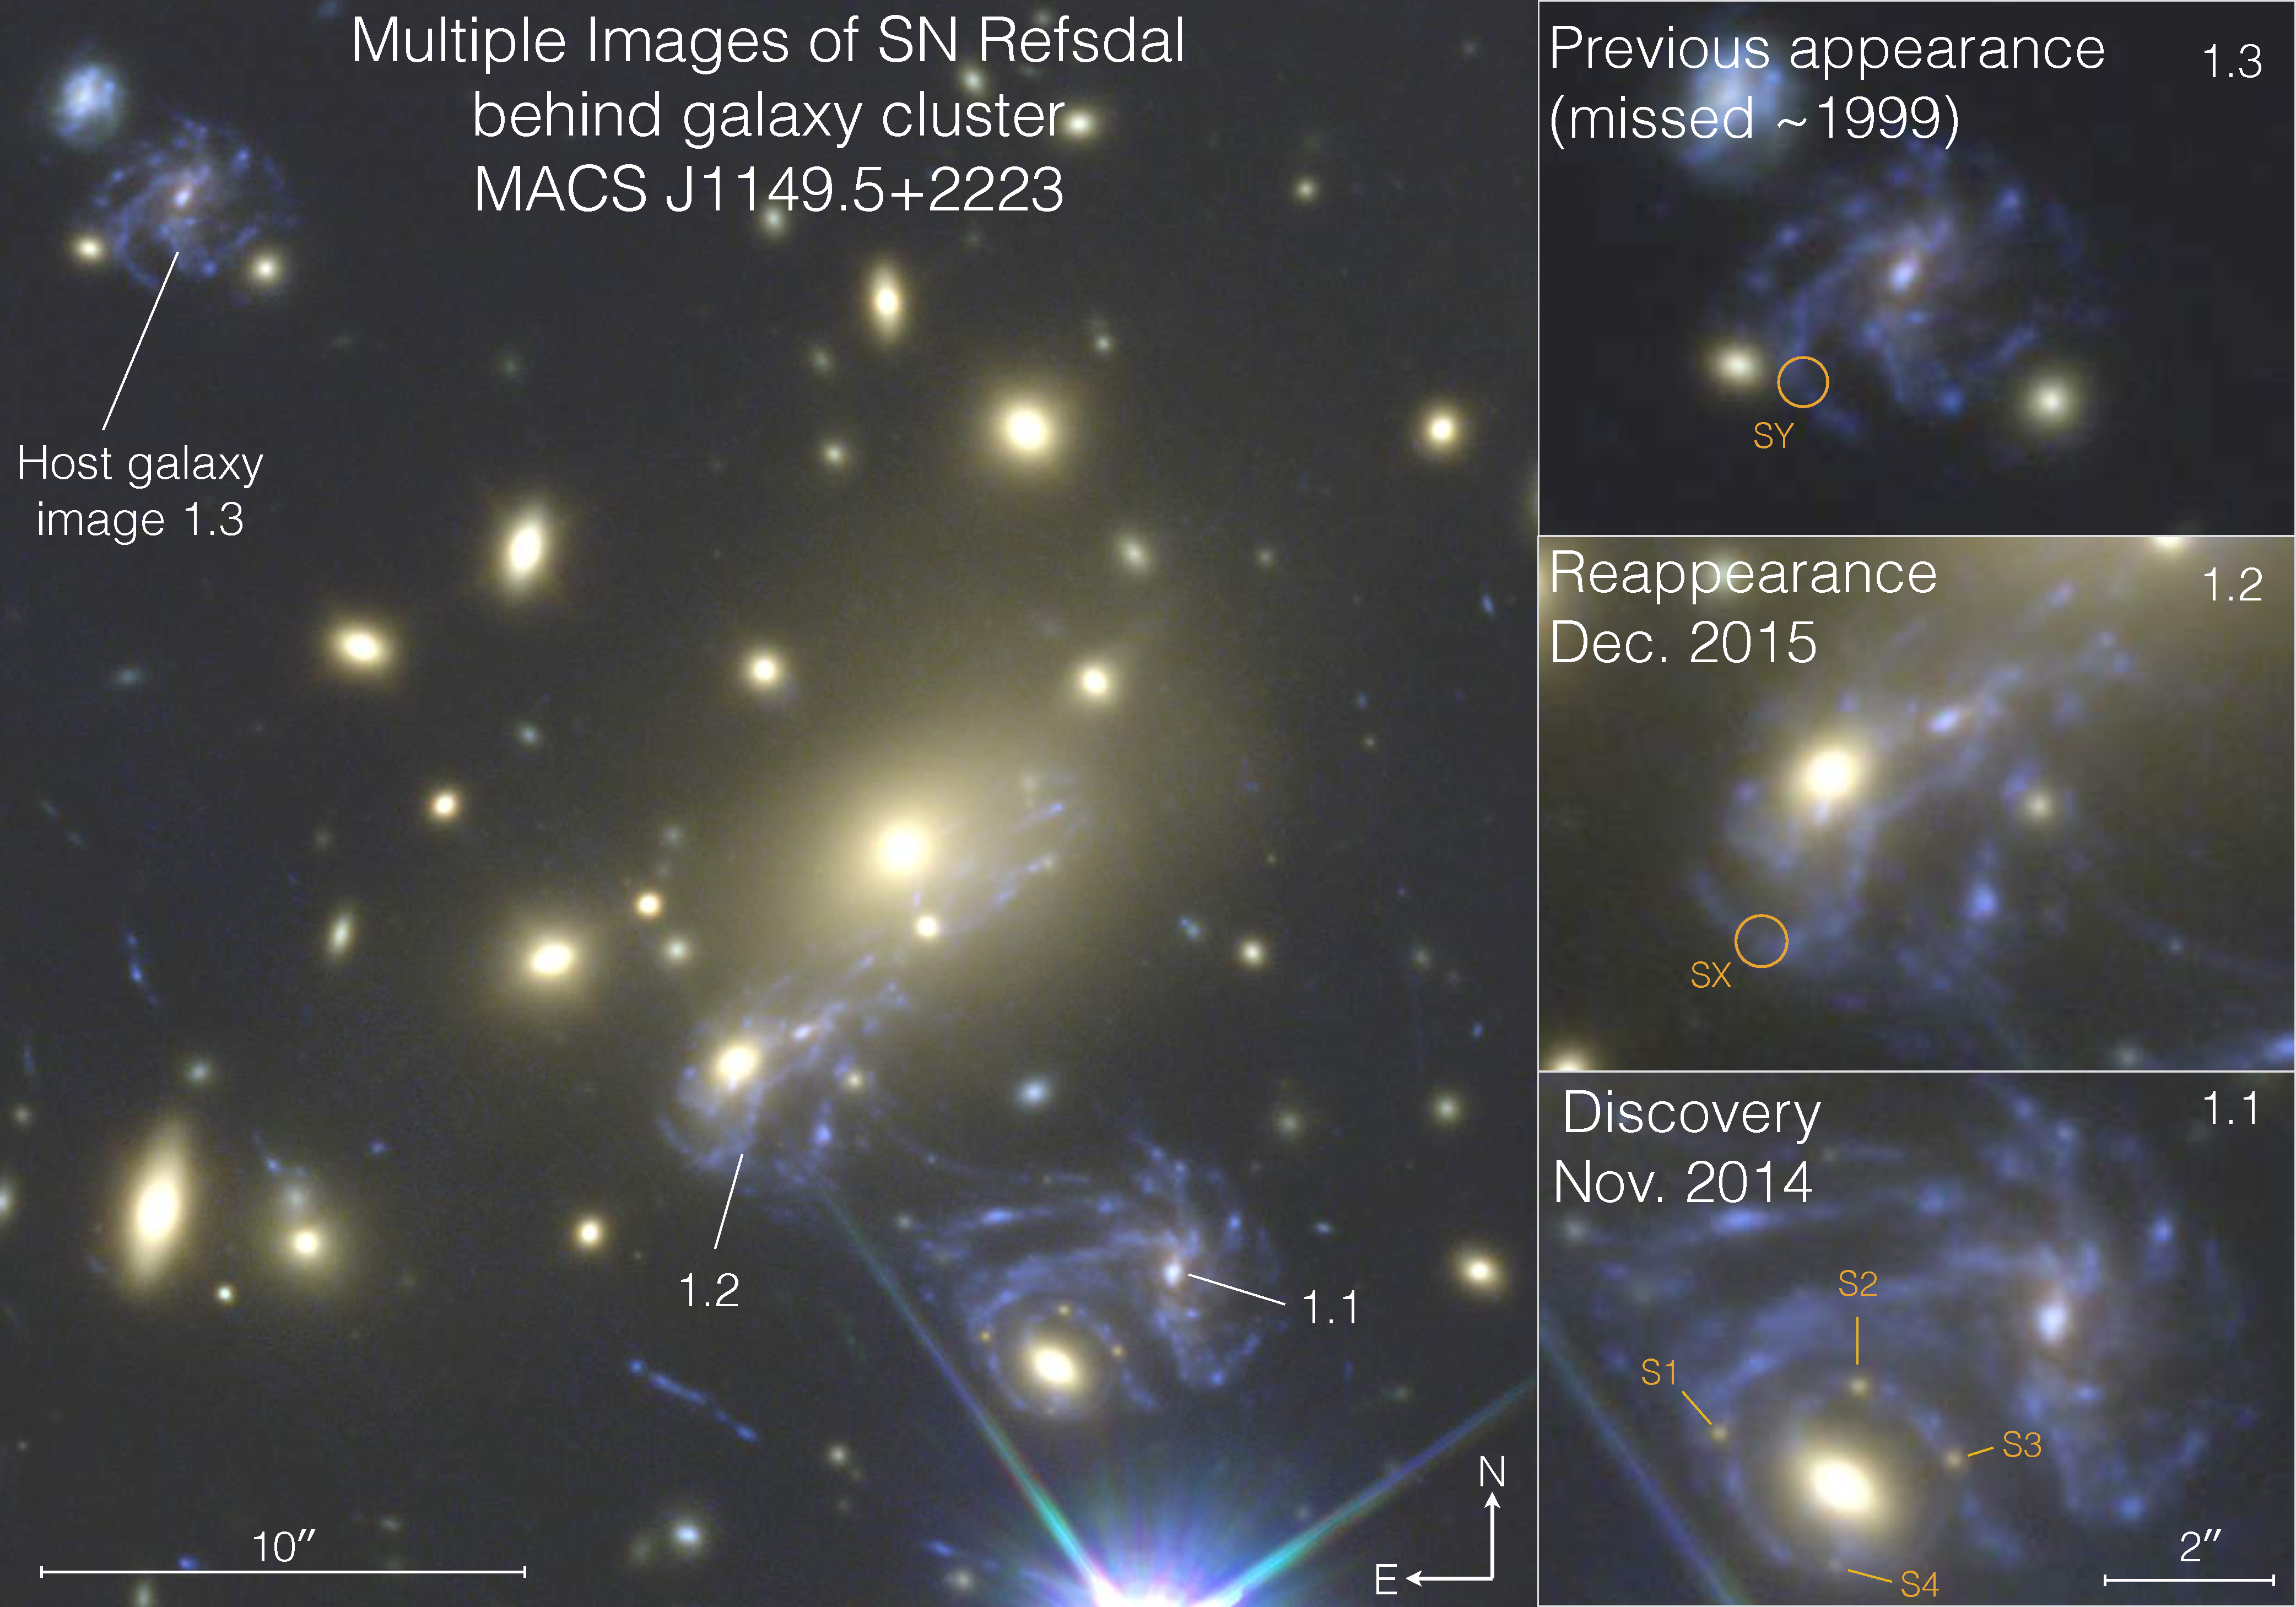
\includegraphics[scale=.15]{refsdal_rodney.pdf}
\caption{MACS J1149.6+2223 field, showing the positions of the three primary images of the SN Refsdal host galaxy (labeled 1.1, 1.2, and 1.3). SN Refsdal appears as four point sources in an Einstein Cross configuration in the southeast spiral arm of image 1.1 (Rodney et al. 2016)}
\end{figure*}


The purpose of this work is to produce an open-source software package called Supernova Time Delays ($\packageName$) that will address the SN modeling needs of the research community and lead to a first-author publication furthering our understanding of lensed SNe. There are currently two software packages, written in Python, which are relevant to this product: Python Curve Shifting (PyCS), and Supernova Cosmology (SNCosmo). PyCS gives users the capability to model quasar light curve data and extract time delays, as well as analyze some lensing and microlensing effects. SNCosmo has extensive SN modeling capabilities and allows for the fitting and sampling of SN light curve data. There will be four components to this research: 1) Integrate SNCosmo and PyCS, giving researchers a tool that can model SN light curve data with the tools present in either software package; 2) Extend the lensing and microlensing algorithm present in PyCS so that it is optimized for SNe; 3) Simulate a large number of SN light curves using SNCosmo and test the ability of $\packageName$ to determine SN parameters; and 4) Explore the abilities of $\packageName$ in analyzing POP III SNe using modeled light curves in anticipation of JWST and WFIRST observations. The final product will be an optimized and accurate tool to fit or simulate SN light curves; classifying a SN and simultaneously measuring redshift, magnification ratios, lensing and microlensing effects, and time delays.


The two software packages described above have many capabilities that are essential to the success of this work. The PyCS package provides powerful tools for analyzing quasar light curves, which we will apply to observed and SNCosmo-generated SN data. Lensed quasars do not have a set of standard underlying light curves, so it is necessary for PyCS to utilize flexible functions such as Chebyshev polynomials or splines to fit quasar light curve data. However, researchers already have a robust set of intrinsic light curve shapes to describe a range of different SN classes; allowing for physically motivated, less flexible models that are much more likely to correctly identify microlensing effects and produce simpler time delay measurements. Therefore, as was done ad hoc in Rodney et al. 2016, $\packageName$ will allow users to fit light curve data using these two separate methods. The PyCS package contains the flexible polynomial method, so it has already been integrated into $\packageName$ (Figure 2). In addition, SNCosmo will be used to generate SN templates from known SN classes with shapes similar to the observed light curve data, allowing certain constraints to float as free parameters. This method will produce a best-fit synthetic light curve, from which time delay, magnifications, SN class, and redshift can be derived. Having these separate tools will allow users to measure parameters using both methods and compare the results, or else simply choose the method that best fits their needs.


\begin{figure}
\centering
\begin{subfigure}{.3\textwidth}
\centering
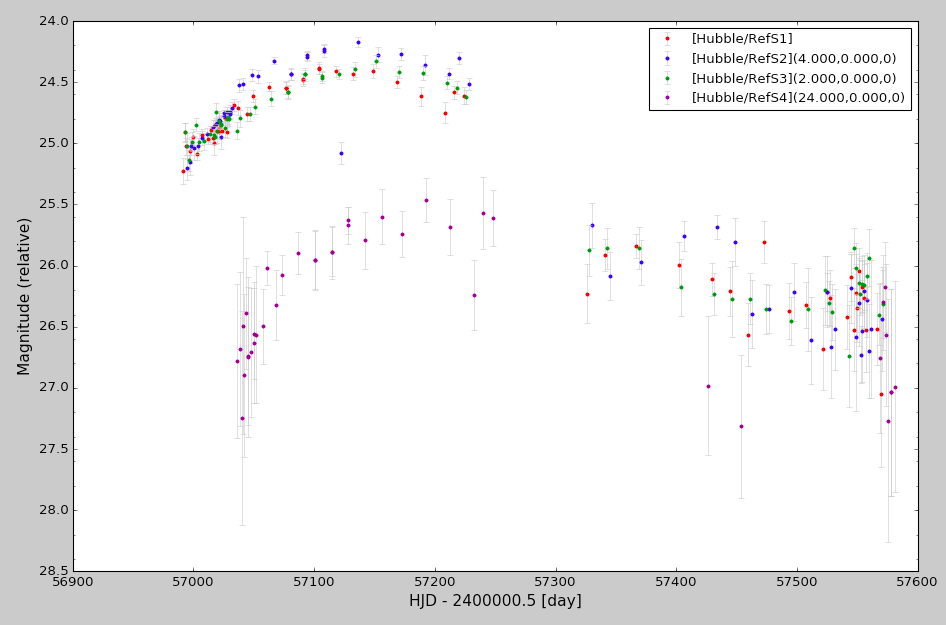
\includegraphics[width=\linewidth]{supcos_points.png}
        \caption{}\label{fig:fig_a}
\end{subfigure}
\begin{subfigure}{.3\textwidth}
\centering
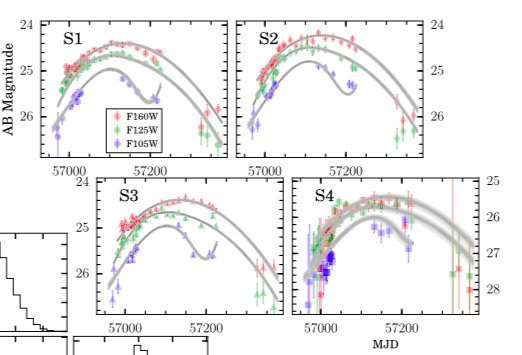
\includegraphics[width=\linewidth]{rodney_fits.png}
\caption{}\label{fig:fig_b}
\end{subfigure}
%\medskip
\begin{subfigure}{.3\textwidth}
\centering
\vspace{0pt}
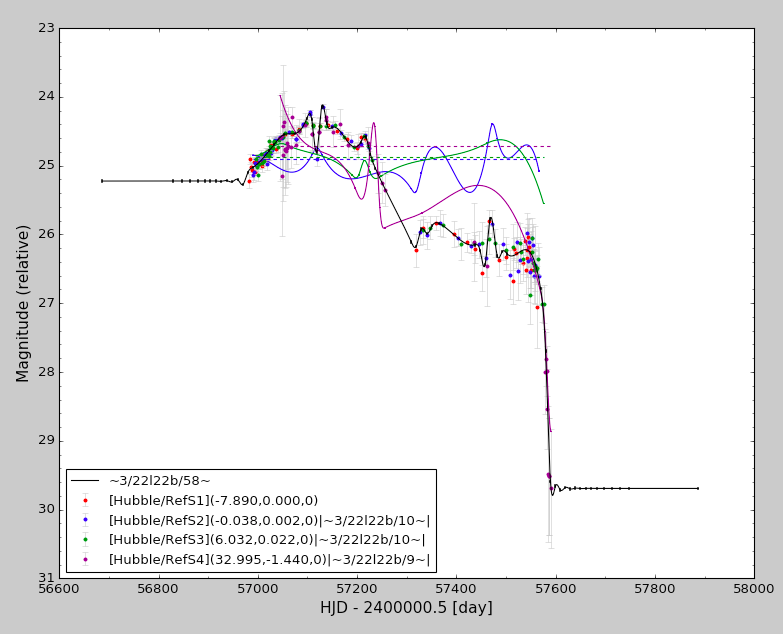
\includegraphics[width=\linewidth]{supcos.png}
\caption{}\label{fig:fig_c}
\end{subfigure}
\caption{a) Colorized are the data representing the four images of SN Refsdal (Figure 1). (b) Results of fitting the SN Refsdal light curves from Rodney et al. 2016 (ad hoc program). (c) Preliminary results from $\packageName$ using a microlensed template from SNCosmo (maybe, or else just spline as it is here and without the microlensing curves) in black. The measured time delays and magnification ratios are in the bottom panel, and are in agreement with the work of Rodney et al. 2016.}
\end{figure}

With no standard software package to use as a tool, the analysis of SN Refsdal ignored the effects of microlensing, which involve small-scale lensing perturbations affecting perhaps only one of the multiple images, as opposed to macro lensing that affects all the images (Rodney et al. 2016). In general, detailed models of multiply imaged SNe are able to successfully match the relative positions of the images, but are frequently unable to correctly reproduce the relative fluxes without accounting for microlensing effects (Dobler and Keeton 2006b). While PyCS currently uses flexible functions to account for microlensing of quasars caused by transverse motion of stars in the lensing galaxy, there is a second form of microlensing unique to lensed SNe. The expanding photosphere of a SN interacts with intervening matter, causing microlensing effects described by Dobler and Keeton 2006a that can exhibit magnitude fluctuations of $\sim$0.2 to $>$0.5 on timescales of weeks to months. This proposed work will seek to include both types of microlensing effects, in addition to macro lensing, in order to increase the precision of time delay measurements. No software package currently exists with this capability, therefore the algorithm will be developed following the methodology of Dobler and Keeton 2006a. 
The $\packageName$ software package, through SNCosmo, is already able to create synthetic SN light curves by varying parameters such as redshift, peak magnitude, intervening dust, and many others (Figure 3). We will therefore generate a wide variety of ``mock'' lensed SNe and subsequently measure the time delays and magnification ratios, which will allow the quantification of the software's accuracy and efficiency. 

%\begin{figure}[h]
%\centering
%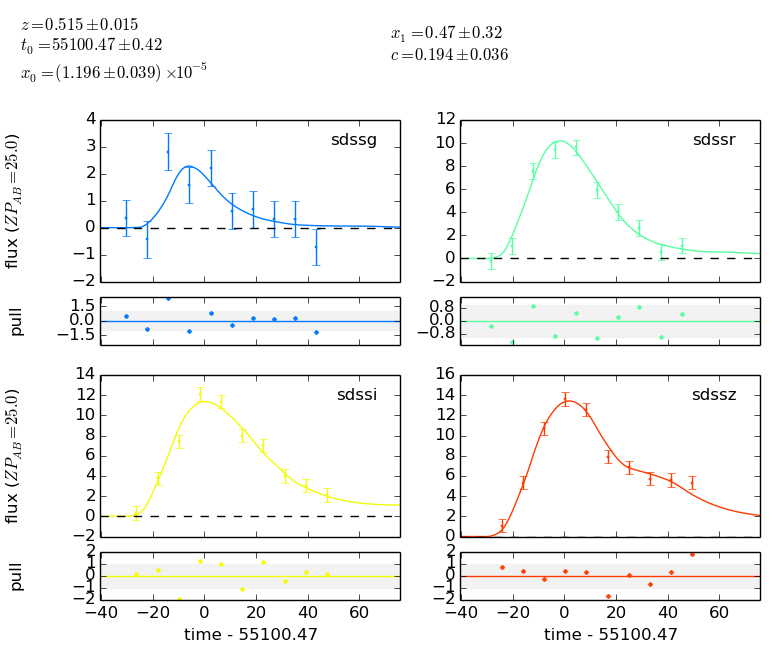
\includegraphics[scale=.4]{sncosmo.png}
%\caption{In addition to spline fitting (Figure 2), $\packageName$ is able to fit model templates to SN light curve data to measure various properties. In future work, the Dobler and Keeton 2006a methodology will be used to extract microlensing effects by identifying perturbations from these templates.}
%\end{figure}

In addition to relatively low redshift SNe, recent simulations of PI SN light curves indicate that various solar mass PI and POP III Type IIn SNe will be visible to both JWST (z$>$30 and z$\sim$-15 respectively) and WFIRST (z$\sim$-20 and z$\sim$-5 respectively) (Magg et al. 2016). Using physically motivated models of the relevant light curves, we will gauge the ability of $\packageName$ to analyze the future observations of these SNe. [This paragraph needs edits or removal]


The $\packageName$ software package will give a standardized, clean, and optimized method of analyzing SN light curve data that is sorely needed in the research community. The package will allow for a broad range of control by the user, including the ability to either use any SN model template from SNCosmo or to generate a template using a different model. $\packageName$ will be able to fit time delay and magnification parameters using either flexible polynomials or light curve templates, simultaneously determining redshift and SN class if they are not already known from other spectra. While many researchers have included the lensing effects of the host galaxy or cluster in their models, $\packageName$ will also identify and account for the two sources of microlensing effects, thereby improving measurement precision. $\packageName$ will be written in Python, a free and open-source programming language, and distributed to SN researchers with extensive documentation including descriptive tutorials. This combination will make $\packageName$ free, widely accessible, and simple to use for anyone in the SN research community.		

The era of JWST will yield an estimated 4-25 new SN observations per field (Mesinger and Johnson 2006), and WFIRST will arrive shortly thereafter in the mid 2020s. Whether it is a follow-up observation of a ground based detection, or a discovery made by one of these space telescopes, having flexible software in place to analyze any SN light curve will be essential to SN cosmologists. Effectively analyzing all of these sources of data from current and future NASA resources is a primary motivation of this work. We expect this research to yield multiple publications about the methodology of the software itself and the simulation results for low and high redshift SNe, as well as advancements in our understanding of lensed SNe resulting from the use of $\packageName$. There are also plans to use this package for follow-up measurements of SN Refsdal and the PTF Type Ia SN parameters, including microlensing effects, making $\packageName$ an invaluable research tool in the SN cosmology community. 

\pagebreak

\begin{figure}[h]
\centering
\includegraphics[scale=.45]{gra_2107_Flow.pdf}
\caption{In addition to spline fitting (Figure 2), $\packageName$ is able to fit model templates to SN light curve data to measure various properties. In future work, the Dobler and Keeton 2006a methodology will be used to extract microlensing effects by identifying perturbations from these templates.}
\end{figure}


\textbf{Works Cited}

Dobler, Gregory, and Charles R Keeton. 2006a. ``Microlensing of Lensed Supernovae.'' Astrophysical Journal.

\

Dobler, Gregory, and Charles R. Keeton. 2006b. ``Finite Source Effects in Strong Lensing: Implications for the Substructure Mass Scale.'' Monthly Notices of the Royal Astronomical Society 365 (4): 1243?62. doi:10.1111/j.1365-2966.2005.09809.x.

\

Goobar, A, R Amanullah, S R Kulkarni, P E Nugent, J Johansson, C Steidel, D Law, et al. 2016. ``The Discovery of the Multiply-Imaged Lensed Type Ia Supernova iPTF16geu,'' 1-24.

\

Kelly, Patrick L, Steven A Rodney, Tommaso Treu, Ryan J Foley, Gabriel Brammer, Kasper B Schmidt, Adi Zitrin, et al. 2015. ``Multiple Images of a Highly Magnified Supernova Formed by an Early-Type Cluster Galaxy Lens.'' Science 347 (6226): 1123-26. doi:10.1126/science.aaa3350.

\

Magg, Mattis, Tilman Hartwig, Simon C O Glover, Ralf S Klessen, and J Whalen. 2016. ``A New Statistical Model for Population III Supernova Rates?: Discriminating Between $\Lambda$ CDM and WDM Cosmologies'' 12 (June): 1-12.

\

Mesinger, Andrei, and Benjamin D Johnson. 2006. ``The Redshift Distribution of Distant Supernovae and Its Use in Probing Reionization'', 80-90.

\

Rodney, S. A., L.G. Strolger, P. L. Kelly, M. Bradac, G. Brammer, A. V. Filippenko, R. J. Foley, et al. 2016. ``SN Refsdal: Photometry and Time Delay Measurements of the First Einstein Cross Supernova'' The Astrophysical Journal 820 (1): 50. doi:10.3847/0004-637X/820/1/50.







